\documentclass[border=5pt]{standalone}
\usepackage{tikz}
\usepackage{amsmath,amssymb,bm}
\usetikzlibrary{arrows.meta, patterns, decorations.pathreplacing}

\begin{document}
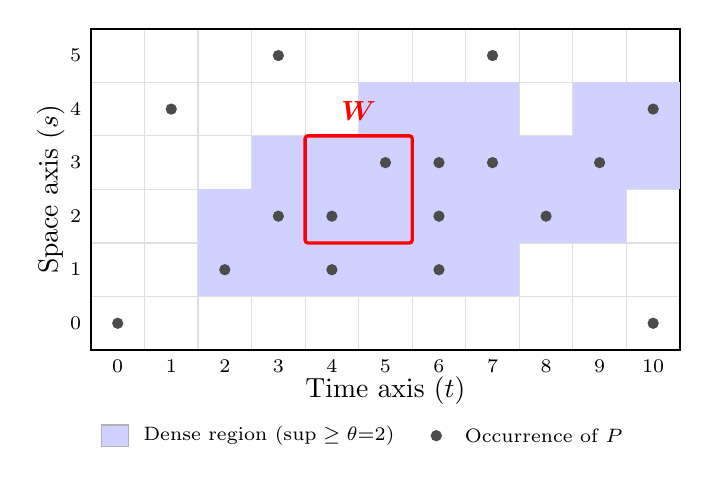
\begin{tikzpicture}[scale=0.68, every node/.style={font=\small}]

% === Grid ===
\draw[gray!25, thin] (0,0) grid[step=1] (11,6);
\draw[thick] (0,0) rectangle (11,6);

% Axis labels
\node[below=6pt, font=\normalsize] at (5.5, 0) {Time axis ($t$)};
\node[rotate=90, above=6pt, font=\normalsize] at (0, 3) {Space axis ($s$)};
\foreach \x in {0,...,10}
  \node[below, font=\scriptsize] at (\x+0.5, 0) {\x};
\foreach \y in {0,...,5}
  \node[left, font=\scriptsize] at (0, \y+0.5) {\y};

% =============================================================
% Dense region in data coordinates
% W=(1,1), theta=2.  Window covers 2x2 cells.
% Dense start points:
%   s_sp=1: t_sp in {2,3,4,5,6}
%   s_sp=2: t_sp in {3,4,5,6,7,8}
%   s_sp=3: t_sp in {5,6,9}
% Dense region (union of 2x2 windows at each dense start):
%   s=0: none
%   s=1: t in {2,3,4,5,6,7}
%   s=2: t in {2,3,4,5,6,7,8,9}
%   s=3: t in {3,4,5,6,7,8,9,10}
%   s=4: t in {5,6,7,9,10}
%   s=5: none
% =============================================================
% s = 1
\foreach \t in {2,3,4,5,6,7}
  { \fill[blue!18] (\t, 1) rectangle ++(1,1); }
% s = 2
\foreach \t in {2,3,4,5,6,7,8,9}
  { \fill[blue!18] (\t, 2) rectangle ++(1,1); }
% s = 3
\foreach \t in {3,4,5,6,7,8,9,10}
  { \fill[blue!18] (\t, 3) rectangle ++(1,1); }
% s = 4 (two separate clusters)
\foreach \t in {5,6,7,9,10}
  { \fill[blue!18] (\t, 4) rectangle ++(1,1); }

% === All occurrences of pattern P (uniform dots) ===
\foreach \t/\s in {
  2/1, 3/2, 4/1, 4/2, 5/3, 6/1, 6/2, 6/3, 7/3, 8/2, 9/3,
  0/0, 1/4, 7/5, 10/0, 10/4, 3/5
}{
  \fill[black!70] (\t+0.5, \s+0.5) circle (3pt);
}

% === Sliding window W (red rectangle) ===
% Example position: start at (t_sp=4, s_sp=2)
% Covers [4,5] x [2,3] = 2 x 2 cells
\draw[red, very thick, rounded corners=1pt]
  (4, 2) rectangle (6, 4);
\node[red, font=\bfseries\normalsize, above] at (5, 4.1)
  {$\bm{W}$};

% === Legend (below grid, single row) ===
\begin{scope}[shift={(0.2, -1.8)}]
  \fill[blue!18] (0, 0) rectangle (0.5, 0.4);
  \draw[gray!60] (0, 0) rectangle (0.5, 0.4);
  \node[right, font=\scriptsize] at (0.6, 0.2)
    {Dense region ($\mathrm{sup} \geq \theta{=}2$)};
  \fill[black!70] (6.25, 0.2) circle (3pt);
  \node[right, font=\scriptsize] at (6.6, 0.2)
    {Occurrence of $P$};
\end{scope}

\end{tikzpicture}
\end{document}
